\section{Sequential designs and heuristic path planning}\label{sec:heuristics}

An important concept underlying this work is the potential of robotic
sampling to adapt survey plans based on data and statistical methods
in accordance with the sense-plan-act control loop
(Fig. \ref{fig:envir1}). We now present a few adaptive strategies for
robotic sampling that build on the notion of EIBV.

\subsection{Background}


\subsection{Optimal Sequential Design}
\label{Optdes}

Our adaptive AUV survey is split into many stages. The selection on
where to sample is constrained by a triangular waypoint graph and
defined by its nearest grid nodes.

Let $d^{j,s}$ denote design number $j$ at stage $s$ of a sequential
survey. For the AUV sampling situation, the choice of design entails a commitment to one of many possible navigation directions on the waypoint graph. Once the choice has been made, the AUV steers in the chosen direction and this entails sampling locations $\bu_{d^{j,s}}$ and data $\by_{d^{j,s}}$ is gathered.  We let
$\mathcal{Y}^{s-1} =\{(d^{*,1}, \by_{d^{*,1}}),\ldots, (d^{*,s-1},
\by_{d^{*,s-1}}) \}$ denote the set of all data gathered until stage
$s-1$ according to selected design $d^{*,1},\ldots,d^{*,s-1}$.  

The design and data define
the conditional GP with mean
$E(\gp[\x]|\mathcal{Y}^{s-1})$ and (cross) covariance matrix
$\mbox{Var}(\gp[\x]|\mathcal{Y}^{s-1})$. These are efficiently updated in a sequential manner keeping track of the mean and covariance kernel of the GP over the stages. As extensions of Eq. \eqref{eq:cokrig} and \eqref{eq:krig:cov}, we have
\begin{eqnarray}\label{eq:krigSUR}
\mu^{s}(\x) &=&\mu^{s-1}(\x)+\lambda^{[s,s]}(\x,\bu_{d^{j,s}})^T (\by_{d^{j,s}}-G_{d^{j,s}} \mu(\x)), \nonumber \\
k^{s}(\x,\x') &=& k^{s-1}(\x,\x')-\lambda^{[s,s]}(\x,\bu_{d^{j,s}})^T K_{Y_{d^{j,s}}} \lambda^{[s,s]}(\x',\bu_{d^{j,s}}),
\end{eqnarray}
where $\lambda^{[s,s]}(\x,\bu_{d^{j,s}})=K^{-1}_{Y_{d^{j,s}}} G_{d^{j,s}} k(\bu_{d^{j,s}},\x)$ and the data covariance is $K^{-1}_{Y_{d^{j,s}}}=G_{d^{j,s}} K^s(\bu_{d^{j,s}},\bu_{d^{j,s}})G^T_{d^{j,s}}+R_{d^{j,s}}$, with measurement model as in Eq. \eqref{eq:meas}.

At stage $s$, the robot must then choose design $d^{j,s}$ where measurements $\by_{d^{j,s}}$ should
be gathered. For the triangularized waypoint
graph all six possible
directions must be evaluated to minimize the expected uncertainty of random sets, and in particular the EIBV for our 
application. We hence focus on choosing designs for data modeled by
Eq. \eqref{eq:meas}, to conduct efficient sequential uncertainty
reduction according to the EIBV criterion. Compared with the
static design $d$ in Eq. \eqref{eq:eibv}, the optimal sequential
design not only considers the best current design grid point, but also
how the data gathered at this node could inform future sampling at
successive stages.

%The optimal path
%selection situation is depicted in Fig. %\ref{fig:PathSelOpt},
%\begin{figure}[b!]
%\centering
%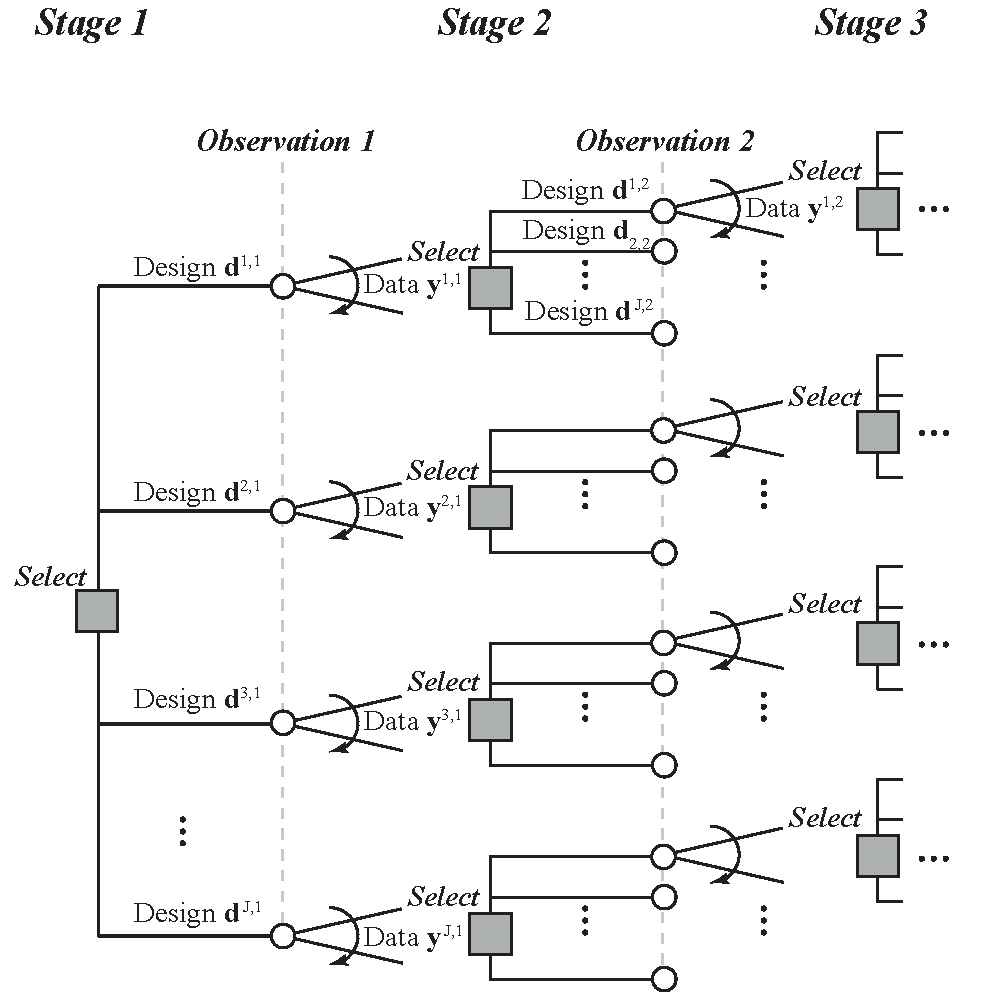
\includegraphics[width=0.85\textwidth]{Figures/sequent_select.pdf}
%\caption{Optimal sequential path selection.}\label{fig:PathSelOpt}
%\end{figure}
%where design choices are indicated by squares while %data realizations are indicated by circles. 
%terms this optimal design is defined as
%\begin{equation}\label{opt_crit}
%    \bd^* = \mbox{argmin}_{d^{j,1}} \left\{ \int_{\by^{j,1}} \mbox{argmin}_{d^{j,2}} \left\{ \int_{\by^{j,2}} \ldots \pi(\by^{j,2}|\by^{j,1}) d\by^{j,2} \right\} \pi(\by^{j,1}) d \by^{j,1} \right\},
%\end{equation}
%where $\ldots$ represents the expected variance reduction in the ES under the continued optimal design, which will depend on the data at earlier stages. 
The mathematical expression for the optimal design involves a series
of intermixed maximizations over designs and integrals over data. In
practice, the optimal solution is intractable because of the enormous
growth over stages (see e.g. \cite{sucar2015probabilistic} and
\cite{powell2016perspectives}).  Instead, we outline heuristic
strategies.


%The derived closed-form solutions for the EIBV are still important building blocks when constructing the sampling designs, as they will be used to score the different adaptive designs. % Efficient
% calculation is important for using adaptive survey designs with
% robotic platforms.
 
\subsection{A Naive Sampling Strategy}
\label{naive}

The simplest heuristic for adaptive sampling is to choose the next
sampling location based on current probabilities. One reduces the
largest levels of uncertainty by selecting the design $j$ with
$P(Z(\x_j) \in T)$ closest to $0.5$.  With temperature and salinity
variables, this {\it{naive}} strategy selects the stage $s$ sampling
design according to:
\begin{eqnarray}\label{critNaive}
    d^{*,s} &=& \mbox{argmin}_{j} |P(Z_1(\x_j) \leq t_1, Z_2(\x_j) \leq t_2 | \mathcal{Y}^{s-1})-0.5|, \nonumber
\end{eqnarray}
where $j$ is indexing all neighboring locations on the waypoint graph.

This strategy does not account for the uncertainty in the GP
variables, but is instead applicable only if one design (node) has EPs
closer to $0.5$ (see Table \ref{tab:sim_rhoab}, row
two). Additionally, this strategy does not account for spatial
correlation. This strategy lacks memory of where it has been and where
the uncertainty has been reduced, and therefore susceptible to local
minima.

\subsection{Myopic Path Planning}
\label{sec:myopic}

The myopic (greedy) strategy which we present here is optimal if we
imagine taking only one more stage of measurements. This selection
strategy is based on expected uncertainty reduction, but it is a
heuristic because there is no anticipation of what the subsequent
designs might offer beyond the first stage.

Based on the currently available data $\mathcal{Y}^{s-1}$, we fit an
updated GP model. Focusing on the EIBV criterion, at the next stage
$s$, the selected design is:
\begin{eqnarray}\label{critSEQ}
    d^{*,s} &=& \mbox{argmin}_{j} \left\{ \int_{\mathcal{M}} E_{\by_{d^{j,s}}|\mathcal{Y}^{s-1}} \left( p(\x;\mathcal{Y}^{j,s})\left( 1-p(\x;\mathcal{Y}^{j,s})\right) \right) d\mes(u), \right\} \\
    p(\x;\mathcal{Y}^{j,s}) &=& P(Z_u \in T |\by_{d^{j,s}},\mathcal{Y}^{s-1}). \nonumber
\end{eqnarray}

Note that this strategy gives a sequential conditional version of
expression (\ref{eq:eibv}). Now $\mathcal{Y}^{s-1}$ is available, and
the expectation is conditional to this data. A similar closed-form
calculation for EIBV is hence applicable in Eq.  \eqref{critSEQ} using the updated
GP model from stage $s-1$ as defined via Eq. \eqref{eq:krigSUR} in the results from Proposition \ref{propo2}. Once the data are collected for the best design $d^{*s}$ at stage $s$, the GP model is updated again. The mean and covariance are used to compute the next design at stage $s+1$, and so on.

Even though this myopic strategy is non-anticipative, it still gives a
reasonable approach for creating designs in many
applications. Moreover, it is easily implemented, in our case, onboard
an AUV, using an efficient data update of the GP model and the
calculation of the closed-form EIBV expressions for each subsequent
trajectory.


\subsection{Look-ahead Trajectory Planning}
\label{sec:LA}

We now extend the myopic strategy to a look-ahead strategy. We consider two stages of
measurements, and the strategy is then optimal in the sense that it accounts consistently for the expectations and minimizations in these two stages, but still without including any planning beyond those two steps. In addition to the
next stage of measurements $\by^{j,s}$, this look-ahead strategy anticipates the subsequent design indexed $j_2$ with data
$\by^{j_2,s+1}$ when choosing the current design $d^{j,s}$. The
selected design is:
\begin{eqnarray}\label{critLA}
    d^{*,s} &=& \mbox{argmin}_{j} \left\{ E_{\by_{d^{j,s}}|\mathcal{Y}^{s-1}} \left( \mbox{argmin}_{j_2}  V_{j_2} \right) \right\}, \\
V_{j_2} & = & \int_{\mathcal{M}} E_{\by_{d^{j_2,s+1}}|\mathcal{Y}^{j,s}} \left( p(\x;\mathcal{Y}^{j,s+1}) ( 1-p(\x;\mathcal{Y}^{j,s+1}) ) \right) d\mes(u), \nonumber \\
    p(\x;\mathcal{Y}^{j,s+1}) &=& P(Z(\x) \in T |\by_{d^{j_2,s+1}},\mathcal{Y}^{j,s}). \nonumber
\end{eqnarray}
Here, $\mathcal{Y}^{j,s}=\{\by_{d^{j,s}},\mathcal{Y}^{s-1}\}$ and
$\mathcal{Y}^{j,s+1}=\{\by_{d^{j_2,s+1}},\mathcal{Y}^{j,s}\}$
represent the sets of data variables, and the expectations are
calculated with respect to the conditional densities given data at
that stage.  We solve the first expectation by Monte
Carlo sampling of data $\by_{d^{j,s}}$ from its conditional
distribution. For each of these data samples, the second expectation
is solved using the closed-form expressions for EIBV using the results from Proposition \ref{propo2}, now with conditioning to the first stage data already going into the mean and covariances in Eq. \eqref{eq:krigSUR}. 

Even though the strategy looks at two sampling stages, it is only used to find
the current best design. When data are collected at stage $s$, the GP model is
updated as in Eq. \eqref{eq:krigSUR}, and the mean and (cross) covariance are
used to compute the next design for stage $s+1$, now anticipating what
stage $s+1$ and $s+2$ could offer, and so on.
This look-ahead approach is much more computationally demanding than
the myopic strategy, so for practical implementation onboard the AUV this is reaching the limits allowed for calculation. We conduct some pruning of the least valuable design paths in the evaluation of Eq. \eqref{critLA}, to get a satisfactory computation time below one minute per waypoint. This means that we use the myopic
strategy to rank the three best designs following the first stage alone, and
for each of these preferred designs, we undertake the look-ahead calculations.

\subsection{Simulation study}
\label{sec:simulations}

\susubsection{Static and Sequential Sampling Designs}
\label{sec:sampling_designs}

%Three different designs are considered as indicated in Figure \ref{fig:stat_design}. 
%\begin{figure}[h!]
%\centering
%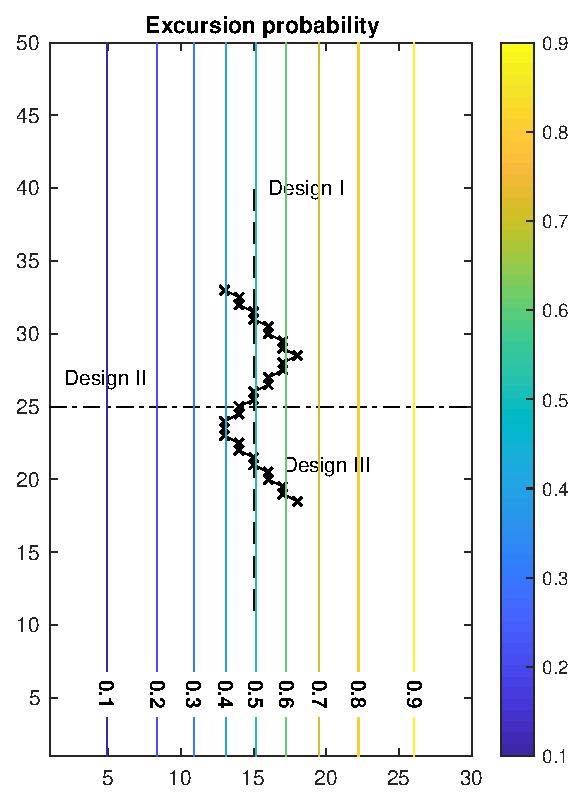
\includegraphics[width=0.65\textwidth]{Figures/Des3.eps}
%\caption{Three different static survey designs plotted on the initial EP.}\label{fig:stat_design}
%\end{figure}
%In this display the designs are plotted along with the prior probability contours of the ES for the reference parameter inputs. 

We compare three different static designs denoted
\textit{static\_north}, \textit{static\_east}, and
\textit{static\_zigzag} with the three described sequential approaches
\textit{naive}, \textit{myopic}, and \textit{look-ahead}. The static
sampling paths are pre-determined and cannot be altered and represent
the pre-planned strategies used in most current AUV operational survey
designs.

For a fixed survey length, a closed-form expression for the EIBV is
available as in Eq. \eqref{eq:eibv}. However, for the sequential
approaches this is not the case. For comparison the properties are
therefore evaluated using Monte Carlo sampling over several replicates
of realizations from the model while conducting simulated sequential
surveys for each one. Fig. \ref{fig:Eprob} shows the conditional EP,
given data gathered along the north-south survey lines in these
displays. In the Monte Carlo replicates, such results are repeatedly
computed to approximate the EIBV. We also compare predictive
performance measured by root mean square error (RMSE) for temperature
and salinity estimates as well as also the variance reduction in these
two variables. It is important to note that the objective function
used by the agent \kc{First of 'agent'. Define it or change it
  to 'robot'? Note further uses below.} is focused on reducing the
EIBV, but we nevertheless expect that we will achieve good predictive
performance for criteria such as RMSE as well. Another non-statistical
criteria that is important for practical purposes is the computational
time needed for the strategy, as this will impact the performance for
an embedded system.

%\begin{figure}[h!]
%\centering
%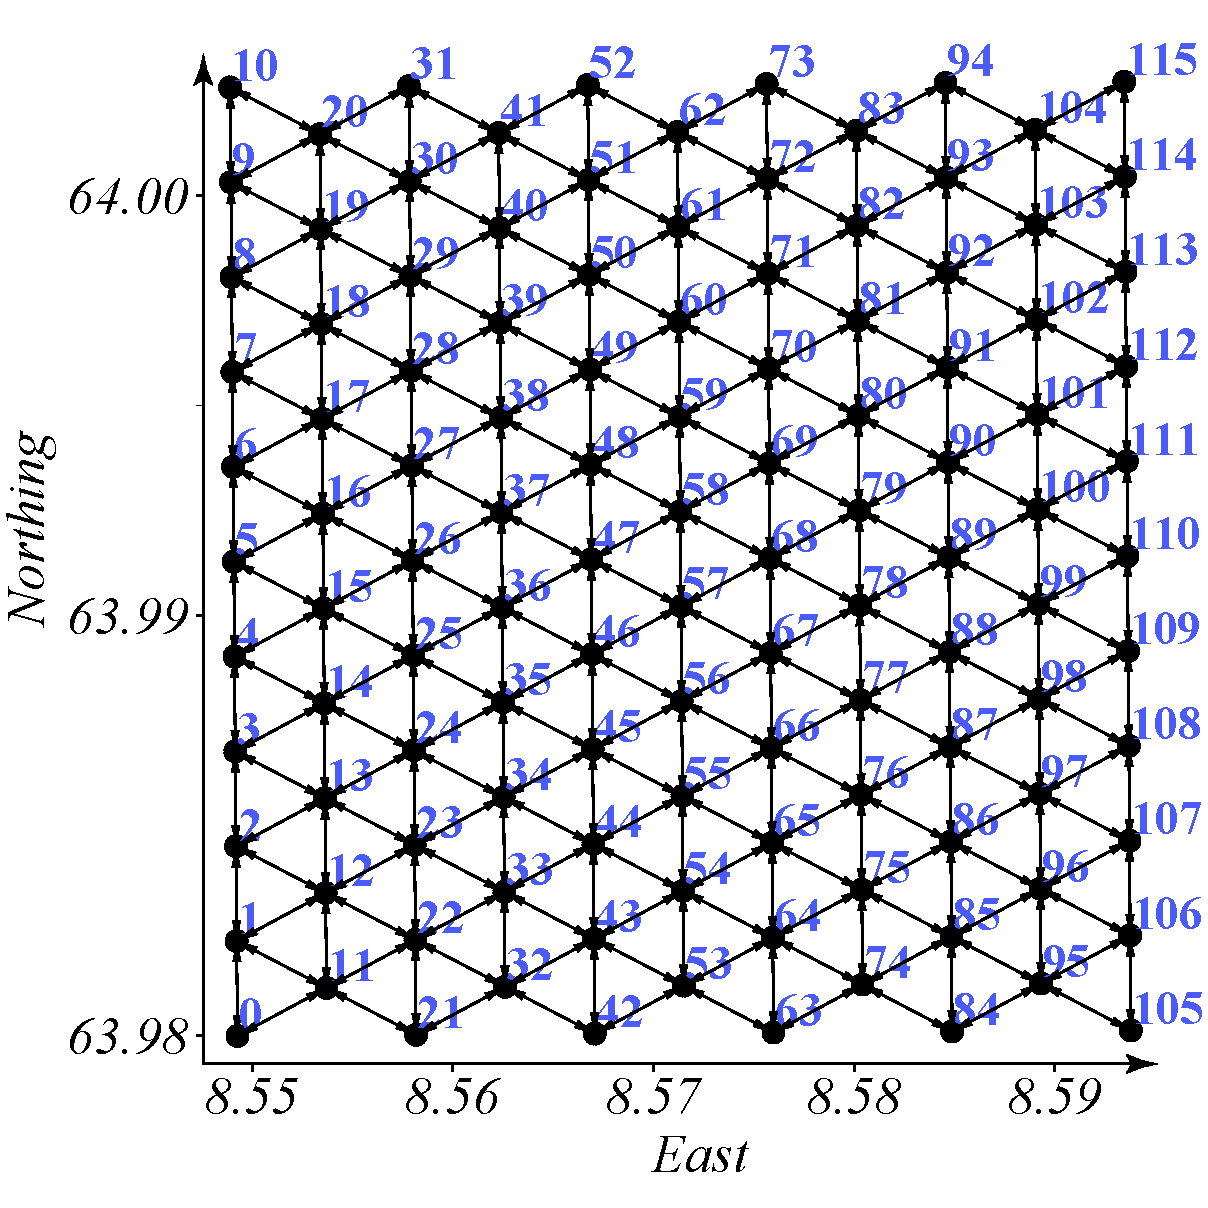
\includegraphics[width=0.50\textwidth]{Figures/sim/wp_graph_paper.pdf}
%\caption{The equilateral waypoint graph used to discretize the
%  trajectory choices over the $31\times31$ grid used to discretize the GP.}
%\label{fig:wp_graph}
%\end{figure}

\begin{figure}[!h] 
\centering 
\subfigure[The waypoint graph.]{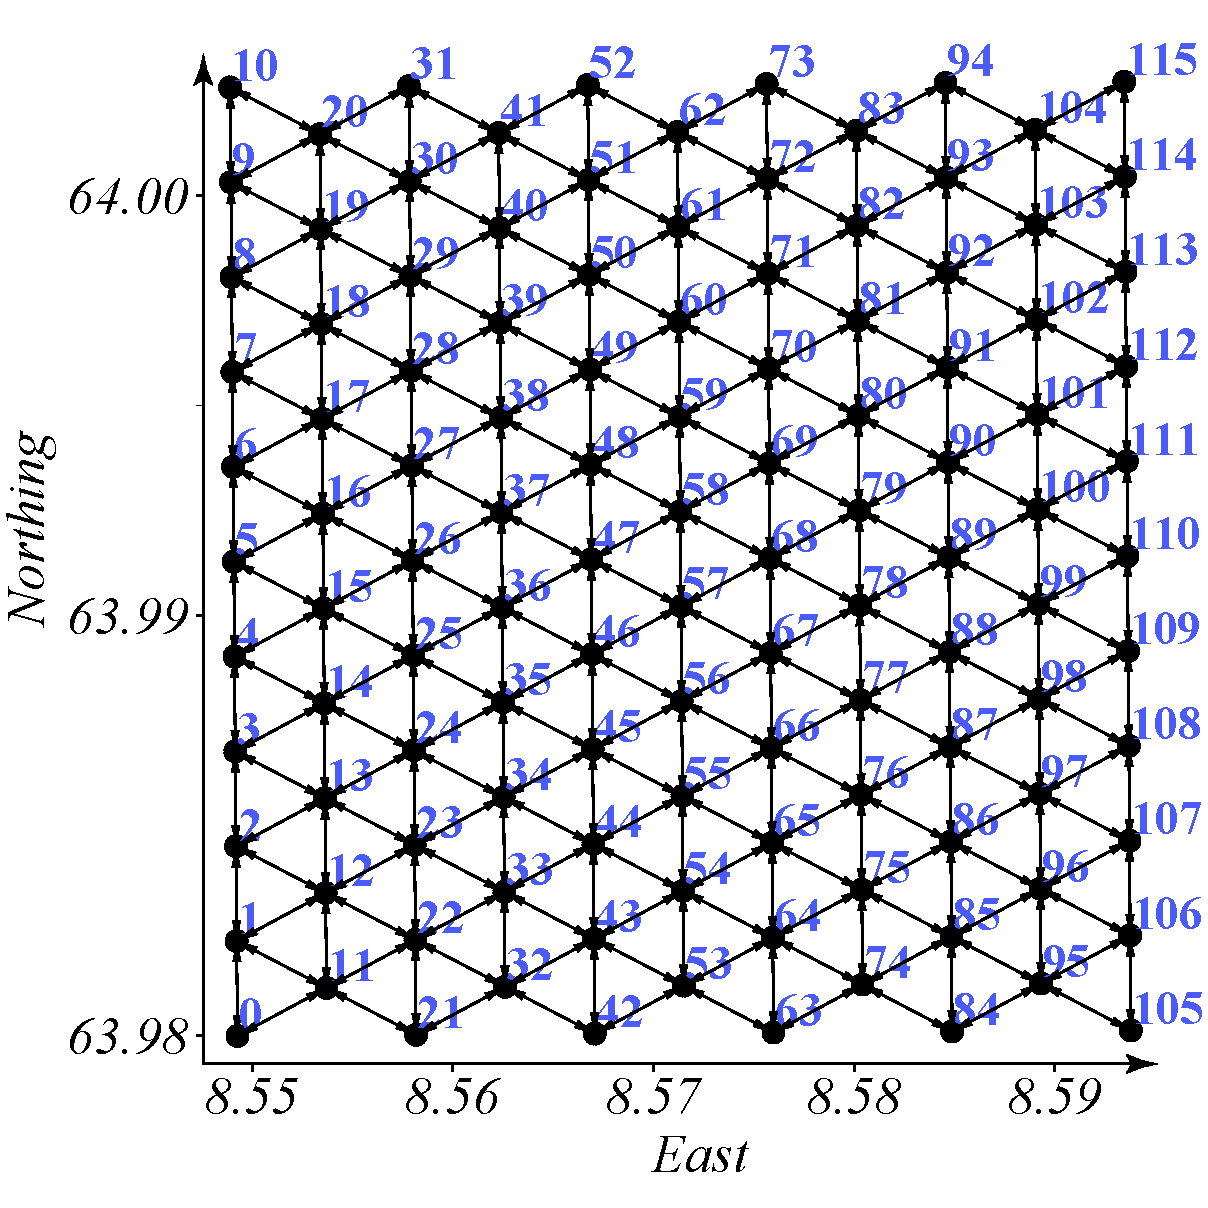
\includegraphics[width =
0.49\textwidth]{Figures/sim/wp_graph_paper.pdf}\label{fig:wp_graph_a}}
\hfill
\subfigure[The waypoint graph in 3D.]{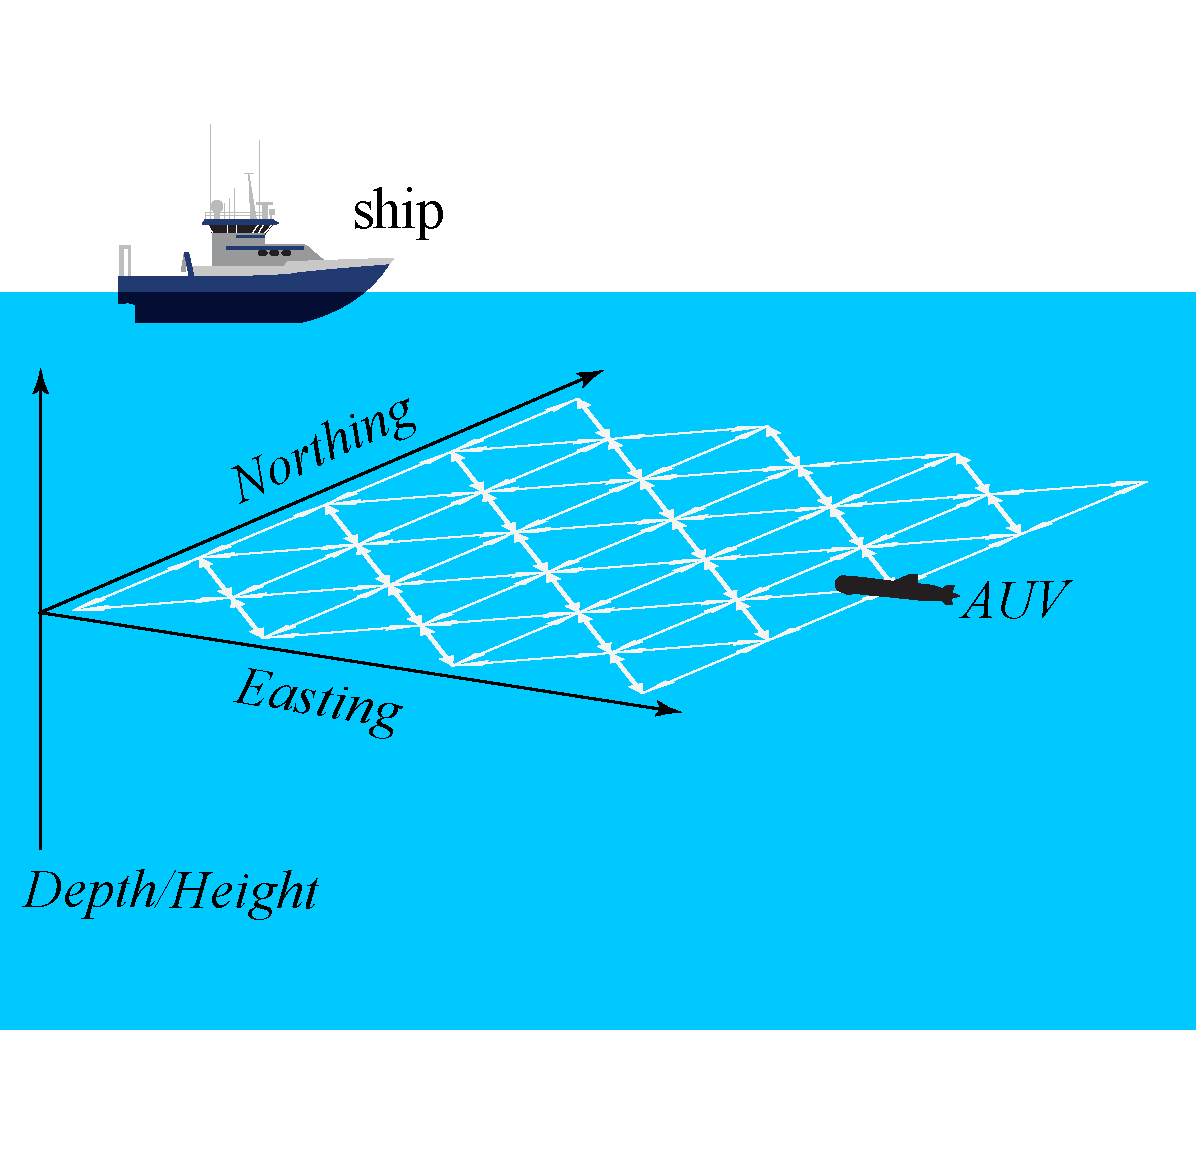
\includegraphics[width =
0.49\textwidth]{Figures/sim/wp_graph_3d.pdf}\label{fig:wp_graph_b}}
\caption{\ref{fig:wp_graph_a} The equilateral waypoint graph used to discretize the
trajectory choices over the $31\times31$ grid used to discretize the GP.
\ref{fig:wp_graph_b} The waypoint grid shown in a 3D environment.}
\label{fig:wp_graph}
\end{figure}

Each strategy is conducted on an equilateral grid as shown in
Fig. \ref{fig:wp_graph}. The sequential sampling agent starts at the
center East-West coordinate at the southern end of the domain (node 53
\kc{Maybe color this node differently and modify the caption?}). The
AUV moves along edges in the waypoint graph while the vehicle makes
measurements. The data is assimilated into the GP model before an
evaluation of the next node to sample is conducted at the end of the
edge.

\subsection{Simulation Results}

A total of 100 replicate simulations were conducted with all
strategies. The results are shown in Fig. \ref{fig:sim_results}, where
the different criteria are plotted as a function of survey
distance. Fig. \ref{fig:avg_ev} shows the resulting drop in IBV for
each of the six strategies. IBV reduction occurs most under the
\textit{myopic} and \textit{look-ahead} strategies, each performing
almost equally; this is expected as the two criteria
(Eq. \eqref{critSEQ} and \eqref{critLA}) are sensitive to differences
in IBV. The \textit{static\_north} design also does well here because
the path is parallel to the boundary between the water masses.

\begin{figure}[h!]
  \centering
  % \subfigure[Excursion set variance $E_{\by}(p[1-p])$.]{\label{fig:avg_ev}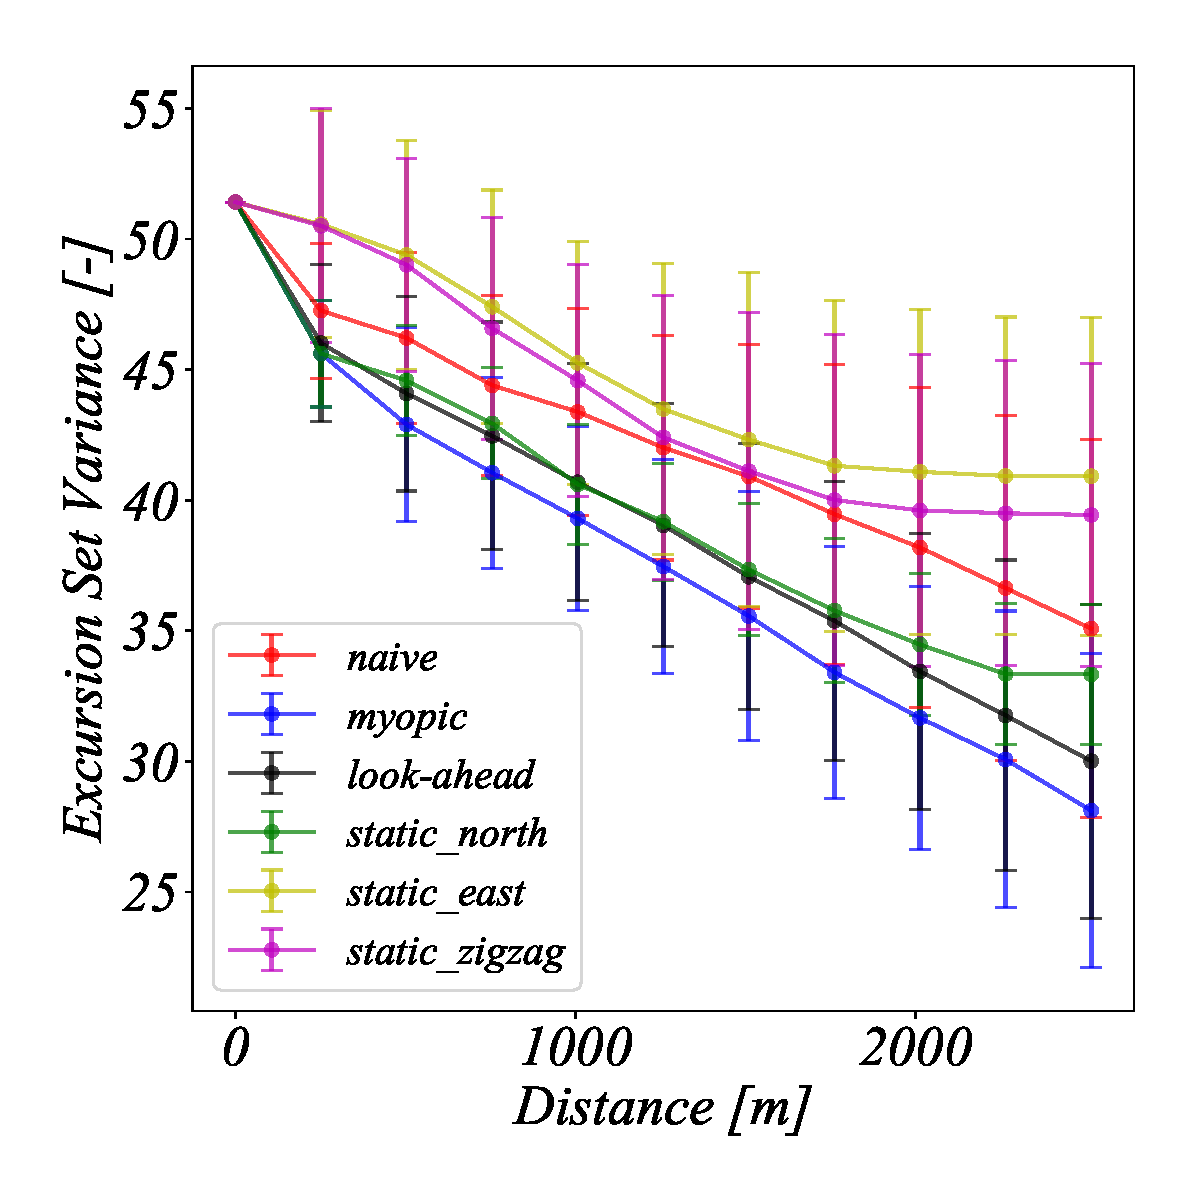
\includegraphics[height=0.49\textwidth]{Figures/sim/avg_EV.pdf}}
  \subfigure[IBV.]{\label{fig:avg_ev}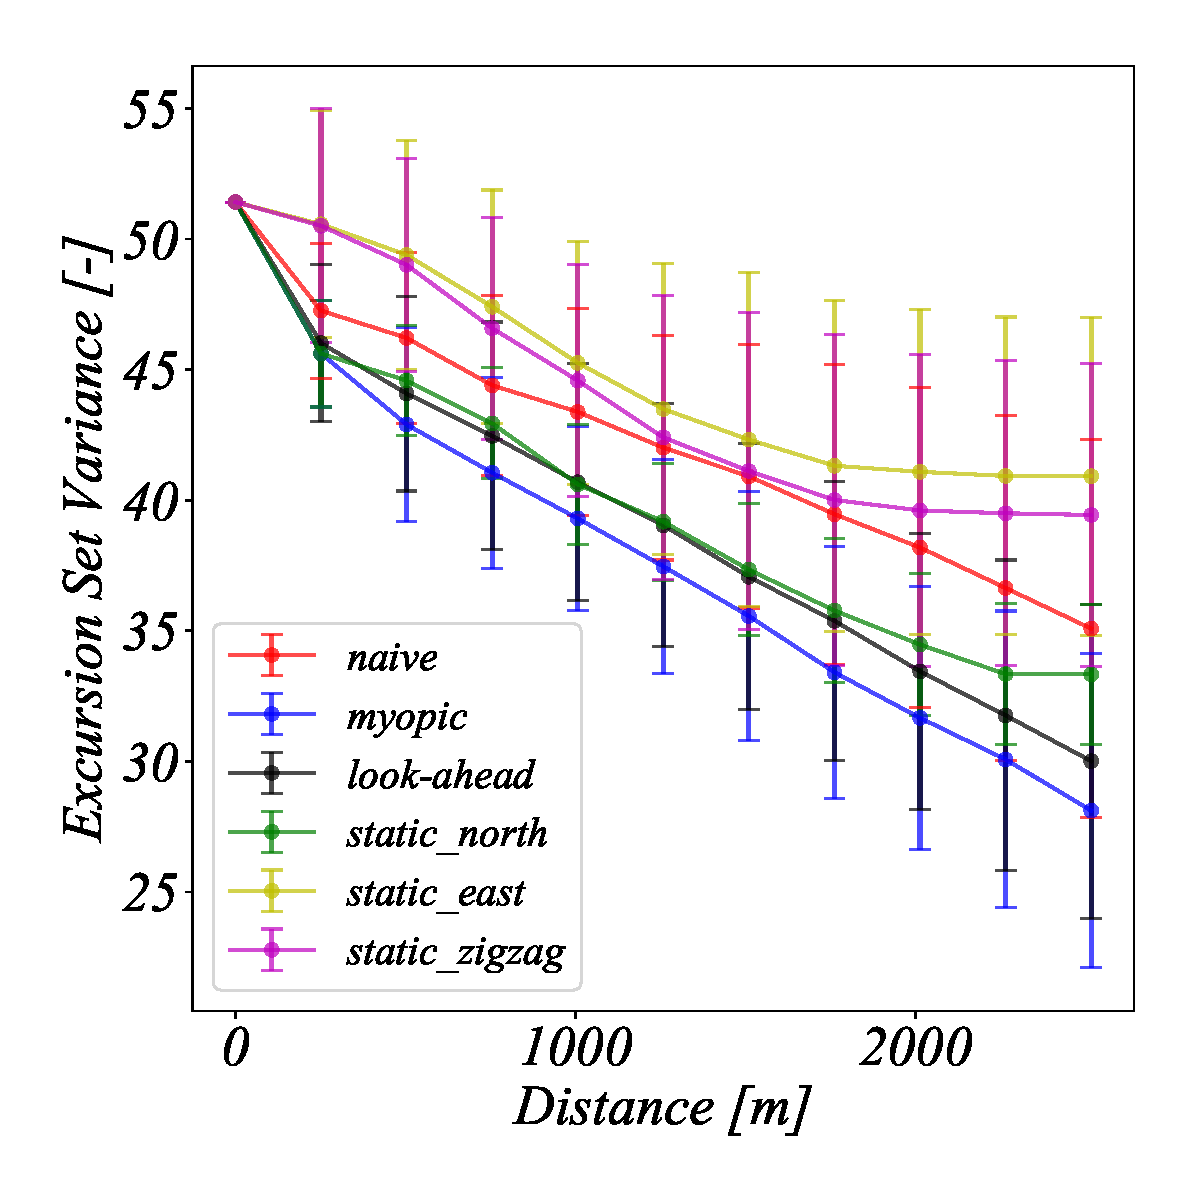
\includegraphics[height=0.49\textwidth]{Figures/sim/avg_EV.pdf}}
  \hfill
  \subfigure[RMSE between estimated field and truth.]{\label{fig:avg_rmse}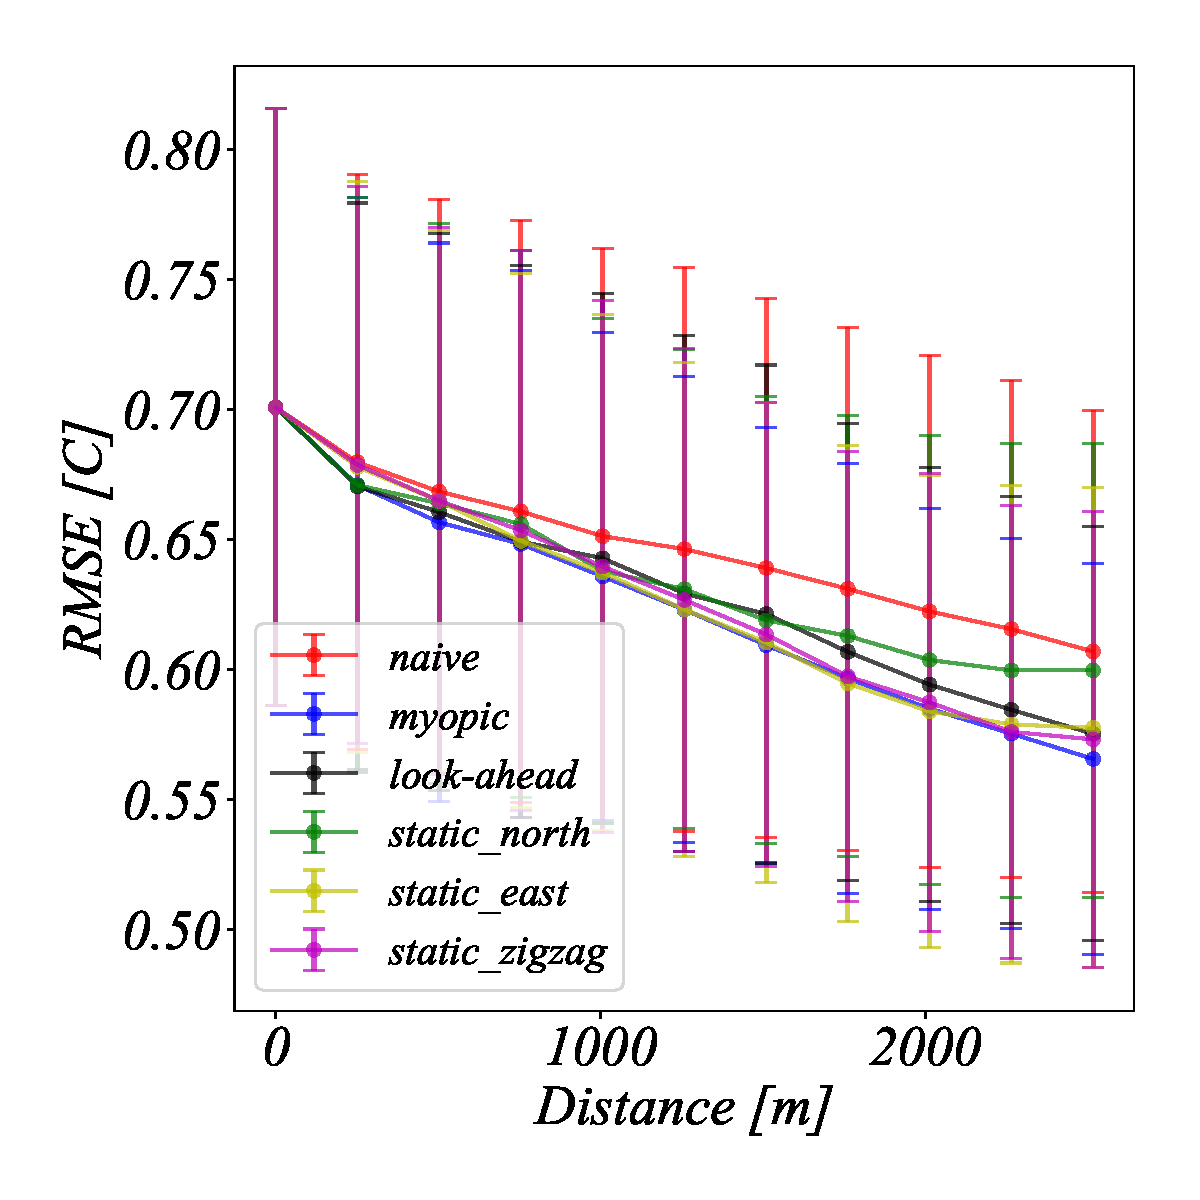
\includegraphics[height=0.49\textwidth]{Figures/sim/avg_RMSE.pdf}}
  \hfill 
  \subfigure[Explained variance $\bR^{2}$.]{\label{fig:avg_r2}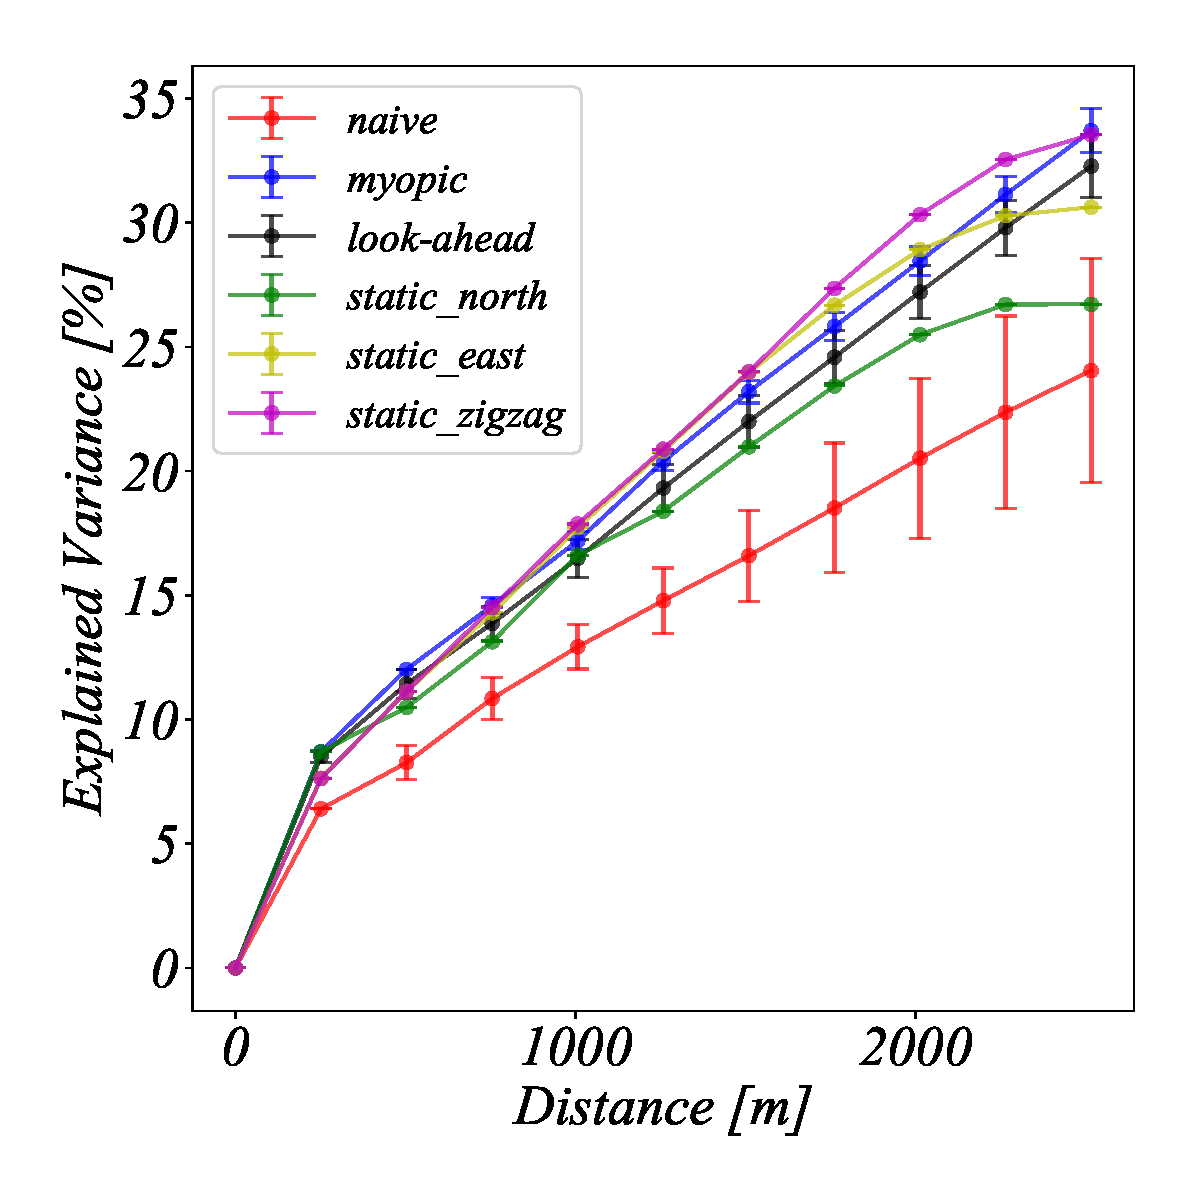
\includegraphics[height=0.49\textwidth]{Figures/sim/avg_R2.pdf}}
  \hfill 
  \subfigure[Computational time for inferencing.\kc{I see only 
    lines associated with 4 variables showing in the graph. Where is
    static\_north and static\_east?}]{\label{fig:avg_time}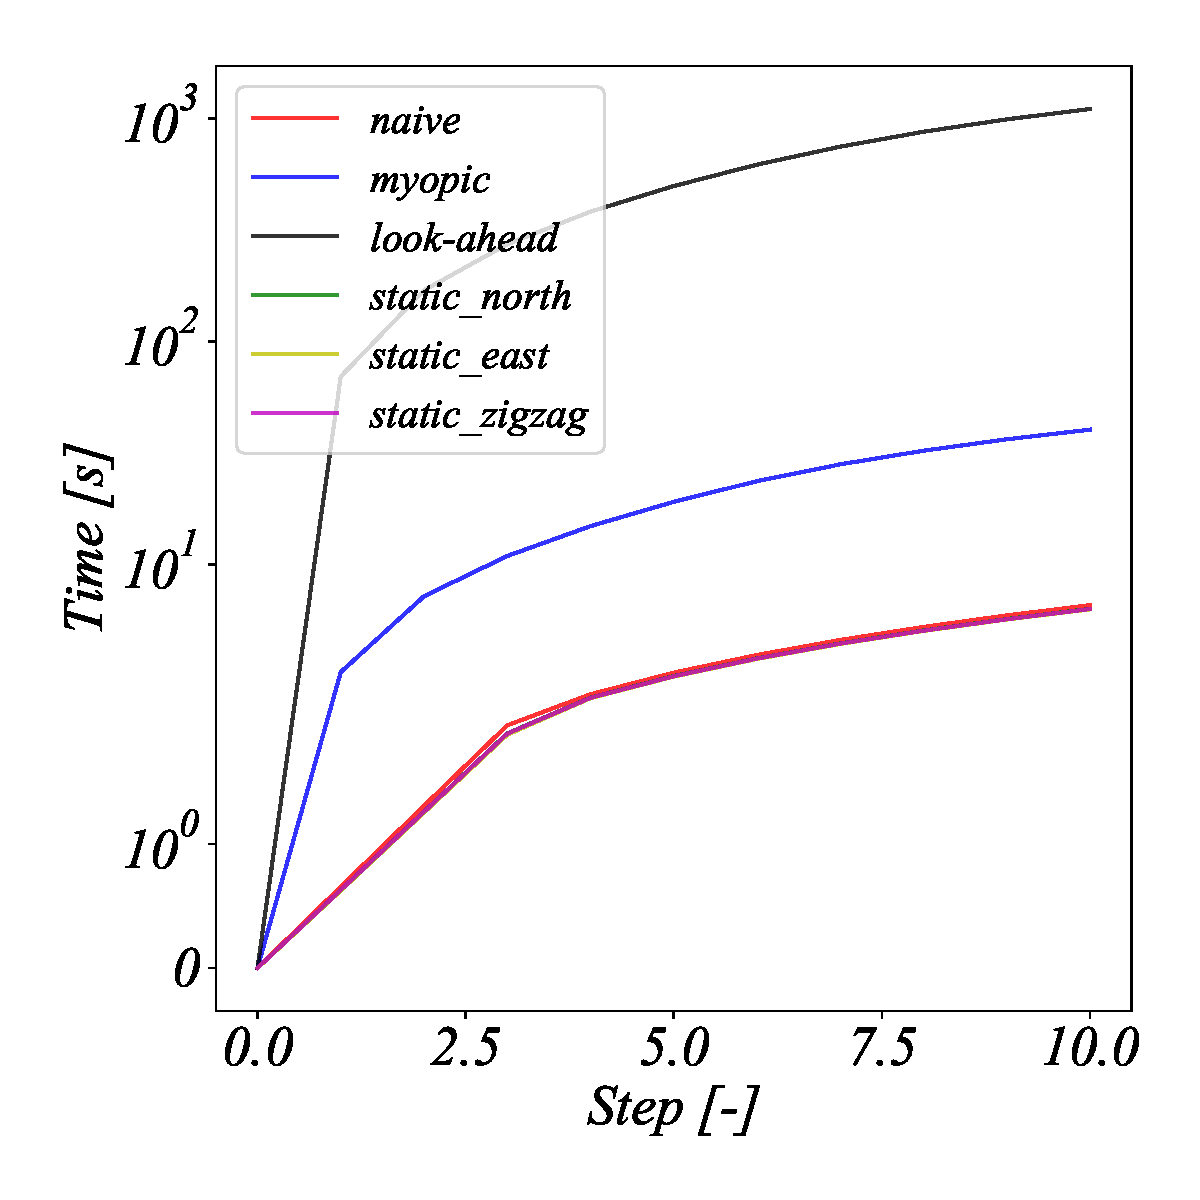
\includegraphics[height=0.49\textwidth]{Figures/sim/avg_Time.pdf}} 
\caption{Simulation results from 100 replicate simulations for 10
  sampling choices/stages on the grid. \kc{Vertical lines show large
    variation in replicate results.}}  
\label{fig:sim_results}
\end{figure}

Fig. \ref{fig:avg_rmse} and \ref{fig:avg_r2} show the resulting drop
in RMSE and increase in explained variance, respectively. Both
\textit{myopic} and \textit{look-ahead} strategies perform well here,
but some of the \textit{static\_east} and \textit{static\_zigzag} also
achieve good results because they are pre-determined to cover large
parts of the domain without re-visitation. Sequential strategies
targeting IBV will sometimes not reach similar coverage, as
interesting data may draw the path into twists and turns. There is
relatively large variety in the replicate results as indicated by the
vertical lines. Nevertheless, the ordering of strategies is similar.


Fig. \ref{fig:avg_time} shows the computational effort: the
\textit{naive} strategy is on par with the static designs, while the
\textit{myopic} strategy is slower. The \textit{look-ahead} is even
slower, reaching levels that are nearly impractical for execution on a
vehicle. Some pruning of the graph is performed to improve the
performance, such as ruling out repeated visitations and
back-and-forth routes. Some of the intermediate results are also
stored for longer planning horizons. Further pruning of branches or
inclusion of other heuristics could be included for better
performance. Then again, the inclusion of heuristics is likely a
contributing factor for the \textit{look-ahead} strategy failing to
outperform the \textit{myopic} strategy.

In Fig. \ref{fig:route_choices}, the realized sampling paths for each
of the sequential schemes and static designs are shown. The
\textit{naive} strategy often gets stuck in the southern part of the
domain because it is too focused on the probabilities near $0.5$. The
\textit{myopic} strategy covers a wider domain than the naive or
look-ahead. There are several reasons for this. First, a greedy
approach will tend to put more emphasis on promising locations close
to the agent, which may lead away from the centre. Second, as the
agent evaluates the impact of locations further away (look-ahead)
where assimilated data has less predictive power, the GP model (which
is centered here) will act to restrict paths deviating from the
central zone.

We studied the sensitivity of the results by modifying the input
parameters to have different correlations between temperature and
salinity, standard deviations, and spatial correlation range.  In all
runs, the \textit{myopic} and \textit{look-ahead} strategies perform
the best in terms of realized IBV, and much better than
\textit{naive}. The \textit{look-ahead} strategy seems to be
substantially better than the \textit{myopic} design only for very
small initial standard deviation or very large spatial correlation
range. \textit{static\_north} continues to be the best static design
for IBV, while \textit{static\_zigzag} is the best design for the
other predictive performance measures, especially so with large
spatial correlation range. We also ran simulation studies with only
temperature data, and for realistic correlation levels between
temperature and salinity, the IBV results are not much worse when only
temperature data are available. In addition to the comparison made in
Table \ref{tab:sim_rhoab}, the current setting includes spatial
correlation and this likely reduces the additional influence of having
bivariate data. However, it seems that having temperature data alone
does a substantially worse job in terms of explained variance